
\begin{table}[h]
    \centering
    \caption{Сравнение времени рендеринга (в секундах) для разных шаблонизаторов}
    \label{tab:rendering-times}
    \begin{tabular}{lrrrr}
        \toprule
        \textbf{Шаблонизатор} & \textbf{100} & \textbf{1000} & \textbf{10,000} & \textbf{100,000} \\
        \midrule
        MLX                   & 0.000117     & 0.000969      & 0.015393        & 0.139218         \\
        TyXML                 & 0.000423     & 0.003726      & 0.026868        & 0.241985         \\
        TyXML\%               & 0.000508     & 0.004809      & 0.033487        & 0.236966         \\
        Dream html            & 0.000041     & 0.001579      & 0.003616        & 0.034738         \\
        Dream eml             & 0.001917     & 0.005415      & 0.040749        & 0.281302         \\
        \bottomrule
    \end{tabular}
\end{table}

% // TODO: доделать график, чтоыб он включал в себя бОльшие величины, а также просто больше величин. Возможно, выделить какие-то особенности других фреймворков.

\begin{figure}
    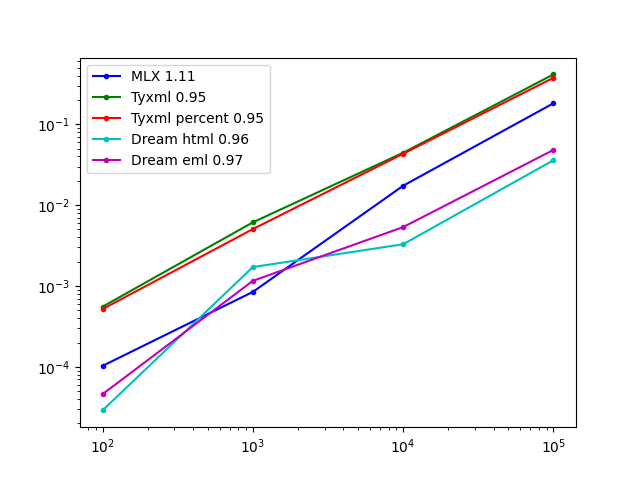
\includegraphics[width=\textwidth]{perfomance.png}
    \label{fig:perfomance}
    \caption{Сравнение производительности шаблонизаторов. График построен с помощью пакета matplotlib. Числа в легенде соответствуют аппроксиммированному углу наклона прямых. Масштаб выбран логарифмическим}
\end{figure}

График построен используя matplotlib python.

Анализ графика: